\chapter{Měření}
Náš projekt se skládá ze dvou částí a to hry a poté měření, které využívá vytvořenou hru pro měření výkonu jednotlivých ECS knihoven. Analýzu tohoto měření jsme provedli v sekci~\ref{benchmark-analysis} a jeho implementaci jsme popsali v sekci~\ref{benchmark-implementation}. V této kapitole si nejprve stanovíme hypotézu, poté si přiblížíme ECS knihovny, které budeme měřit a na závěr si prezentujeme výsledky tohoto měření.

\section{Hypotéza}
\label{chap:hypothesis}
V této sekci si stanovíme hypotézu našeho měření. V našem měření měříme jak dlouho trvá odsimulovat určitý počet iterací naší hry s jednotlivými ECS knihovnami. Ty se dají rozdělit na kategorie podle určitých vlastností. V této kapitole stanovíme jak si myslíme, že se jednotlivé kategorie umístí.

% Do teď jsme se věnovali samotné hře, kterou v následujících kapitolách budeme chtít použít pro porovnání výkonu ECS knihoven. Ale ještě předtím, konkrétně v této kapitole, si rozebereme předpokládané výsledky tohoto porovnání.

\subsection{Cache}
Využití cache je klíčový faktor pro výkon ECS knihovny, proto si nyní připomene co to vlastně je a jak funguje.

Program si svoje data uchovává v paměti RAM. Ovšem přístup do této paměti je z hlediska času drahý. Pro představu u moderních pamětí takovíto přístup může trvat vyšší desítky nanosekund. Z tohoto důvodu se využívají menší paměti, takzvané cache, které disponují mnohem vyšší rychlostí ale mnohem menší velikostí. Pro představu moderní procesory používají cache, u kterých přístup může trvat menší desetiny nanosekund.

Při přístupu k datům se procesor nejprve podívá zda nemá data již v této cache. Pokud ano, jedná se o takzvaný \textit{cache hit} a data si z ní načte. Pokud ne, jedná se o takzvaný \textit{cache miss} a je nutné data načíst z hlavní paměti. 

Již víme, že \textit{cache miss} jsou drahé, proto je potřeba pro vysoký výkon je minimalizovat. Ale jak přesně procesor rozhoduje o tom, jaká data budou v cache a jaká ne. Využívá se takzvané \textit{časové} a \textit{prostorové lokality}. \textit{Časová lokalita} spočívá v tom, že pokud jsme přistoupili k nějakým datům, je velká šance, že k nim brzo budeme chtít přistoupit znovu. Nadruhou stranu \textit{prostorová lokalita} spočívá v tom, že pokud jsme přistoupili k nějakým datům, je velká šance, že budeme chtít přistoupit také k datům, které se nacházejí blízko nich.

Jedna z možností, jak minimalizovat počet \textit{cache miss}, je využít sekvenčního přístupu. Pokud budeme přistupovat k datům, které jsou v paměti hned za sebou, tak díky \textit{prostorové lokalitě} bude počet \textit{cache miss} velmi malí.

Je nutné upozornit, že výše popsaný model cache je úmyslně zjednodušen. Velice detailní popis cache lze nalézt v \textit{Cache Memories}~\cite{10.1145/356887.356892} od \textit{Alana Jaye Smitha}. Stručnější popis a také informace o tom jak lze cache využít lze nalézt v již zmiňované knize \textit{Game Programming Patterns}~\cite{nystrom2014game}, konkrétně v kapitole \textit{Data Locality}. 

\subsection{Arch type}
Některé ECS knihovny pro lepší výkon používají \textit{arch type}. Jedná se o datovou strukturu pro ukládání komponent. Knihovny, které používají tuto datovou strukturu mají většinou velký výkon, proto před stanovením hypotézy si použití \textit{arch type} lehce přiblížíme.

Jak již bylo zmíněno, \textit{arch type} je datová struktura. Tato datová struktura představuje typ entity. Tento typ je jednoznačně určen typy všech komponent dané entity. Je možné si jej představit jako tabulku, kde jednotlivé sloupečky odpovídají komponentám a v každém řádku se nacházejí instance komponent pro danou entitu. Například můžeme mít \textit{arch type} vyobrazený v tabulce~\ref{tab:arch-type}. Tento \textit{arch type} je jednoznačně určen typy komponent \texttt{Position} (představující pozici entity), \texttt{Health} (představující počet životů entity) a \texttt{Damage} (představující poškození, které entita může udělit jiné entitě).

\begin{table}[!htb]
    \centering\footnotesize\sf
    \begin{tabular}{c c c c}
        \toprule
        entita & \texttt{Position} & \texttt{Health} & \texttt{Damage} \\
        \midrule
        hráč & $(0,0)$ & 10 & 3 \\
        nepřítel & (5,4) & 6 & 1 \\
        npc & (-4,8) & 16 & 9\\
        \bottomrule
    \end{tabular}
    \caption{Tabulka vyobrazující \textit{arch type}, který je jednoznačně určen komponentami \texttt{Position}, \texttt{Health} a \texttt{Damage}. Tento \textit{arch type} obsahuje tři entity, konkrétně hráče, nepřítele a npc.}
    \label{tab:arch-type}
\end{table}

Jednotlivé \textit{arch type} jsou uloženy ve \textit{world}. Každý \textit{arch type} má v sobě několik polí, konkrétně jedno pole pro každý typ komponenty. V každém poli jsou poté uloženy instance příslušných komponent. V případě \textit{arch type} z tabulky~\ref{tab:arch-type} by tento \textit{arch type} obsahoval jedno pole pro \texttt{Position} komponenty, jedno pole pro \texttt{Health} komponenty a jedno pole pro \texttt{Damage} komponenty.

Pokud bychom chtěli iterovat přes všechny entity s danými komponentami, stačilo by nám projít příslušná pole všech \textit{arch type} s těmito komponentami. Tato iterace by byla, díky sekvenčnímu přístupu zmíněnému v minulé sekci, velice rychlá. Ke \textit{cache miss} by docházelo pouze při přechodu na další \textit{arch type}.

Nevýhodou knihoven založených na \textit{arch type} bývá pomalé přidávání a odebírání komponent. Pokud je entitě přidána nebo odebrána komponenta, dojde ke změně jejího \textit{arch type}. Při této změně se vezmou instance všech komponent dané entity a přesunou se do nového \textit{arch type}.

Pro více informací o \textit{arch type} a o tom jak je ECS knihovny využívají je možné nahlédnout do série článků \textit{ECS back and forth}~\cite{Caini_2019} od Michela Cainiho.

\subsection{Hypotéza}
\label{hypothesis}
Nyní vyřkneme hypotézu. Jednotlivé ECS knihovny lze rozdělit do kategorií na základě jistých vlastností. My tyto kategorie popíšeme a stanovíme jaké bude jejich pořadí při výkonnostním porovnání.

Nejrychleji vyjdou ECS knihovny, které používají \textit{arch type}. Jak již bylo zmíněno, \textit{arch type} je datová struktura s kterou lze, díky malému počtu \textit{cache miss}, dosáhnout velkého výkonu při iteraci entit. Z těchto důvodů ECS knihovny, které \textit{arch type} používají vyjdou nejlépe.

Některé ECS knihovny vyžadují aby jednotlivé komponenty byli reprezentovány jako třídy. Tyto knihovny vyjdou nejhůře. V případě, že komponenta je třída, znamená to, že její proměnné musejí být pointery. Z toho důvodu iterace přes komponenty v těchto knihovnách vede ve velmi velký počet \textit{cache miss}, kvůli kterému se tyto knihovny umístí nejhůře. 

Zbývají knihovny, které povolují komponenty reprezentovat jako struktury, ale zároveň nepoužívají \textit{arch type}. Tyto knihovny se umístí hůře než knihovny, které používají \textit{arch type}, ale lépe než knihovny, které vyžadují aby komponenty byli třídy.

\section{Měřené knihovny}
V této sekci se budeme zabývat ECS knihovnami, které budeme měřit. První si uvedeme odkud měřené ECS knihovny bereme a poté si jednotlivé ECS knihovny krátce představíme.

V sekci~\ref{sec:ecs-libs} jsme zmínili, že existuje repositář \textit{EcsCsharpBenchmark}~\cite{EcsCsharpBenchmark} na platformě GitHub obsahující výkonnostní porovnání ECS knihoven pro C\#. Tento repositář byl inspirací této práce, která také porovnává jednotlivé ECS knihovny, ale na místo jednoduchých testů je porovnává na hře. V našem měření budeme měřit knihovny, které byli porovnávány ve zmiňovaném repositáři \textit{EcsCsharpBenchmark}~\cite{EcsCsharpBenchmark}.

Od zahájené této práce byl repositář \textit{EcsCsharpBenchmark}~\cite{EcsCsharpBenchmark} několikrát upraven. Během úprav byli přidávány a odebírány některé ECS knihovny z porovnání. V této práci se zaměříme na knihovny, které byli v repositáři \textit{EcsCsharpBenchmark}~\cite{EcsCsharpBenchmark} porovnávány během commitu \textit{db67d1d}~\cite{EcsCsharpBenchmarkCommit}.

Nyní si představíme jednotlivé ECS knihovny, které budeme měřit. U každého si uvedeme přeložený popisek, který je možné nalézt v repositáři dané knihovny. Tyto popisky jsou doslovně převzaté a autor práce neručí za korektnost informací, které jsou jejich obsahem.

\begin{enumerate}
    \item \textbf{Arch~\cite{Arch}:} Vysoko-výkonnostní ECS knihovna založená na Archtype určená pro herní vývoj a data-oriented programování.
    \item \textbf{DefaultEcs~\cite{DefaultEcs}:} ECS framework, který si klade za cíl být přístupný s minimálními omezeními, zatímco zachovává co největší výkon pro vývoj her.
    \item \textbf{Entitas~\cite{Entitas}:} Nejpopulárnější open-source ECS framework pro C\# a Unity.
    \item \textbf{HypEcs~\cite{HypEcs}:} Lightweight a snadno použitelná ECS knihovna s efektivní sadou funkcionalit pro tvorbu her.
    \item \textbf{LeoECS~\cite{LeoECS}:} Lightweight ECS framework pro C\#. Mezi hlavní cíle tohoto frameworku patří výkon, nulová nebo minimální alokace, minimalizace využití paměti a absence závislostí na jakémkoliv herním enginu. (Přeloženo přes ChatGPT.)
    \item \textbf{LeoEcsLite~\cite{LeoEcsLite}:} Lightweight ECS framework pro C\#. Mezi hlavní cíle tohoto frameworku patří výkon, nulová nebo minimální alokace, minimalizace využití paměti a absence závislostí na jakémkoliv herním enginu. (Přeloženo přes ChatGPT.)
    \item \textbf{MonoGameExtended.Entities~\cite{MonoGameExtended}:} Moderní vysoce výkonnostní ECS framework založený na Artemis.
    \item \textbf{RelEcs~\cite{RelEcs}:} Lightweight a snadno použitelná ECS knihovna s efektivní sadou funkcionalit pro tvorbu her.
    \item \textbf{Svelto.ECS:} Reálný ECS framework pro C\#. Umožňuje psát zapouzdřený, oddělený, udržovatelný, vysoce efektivní, datově orientovaný, cache-přátelský kód bez bolesti.
\end{enumerate}

\section{Výsledky}
Analýzu měření jsme provedli v sekci~\ref{benchmark-analysis}. Poté v sekci~\ref{benchmark-implementation} jsme si rozebrali implementaci měření. V této sekci se budeme věnovat výsledkům tohoto měření.

Předtím něž si prezentujeme výsledky měření, tak si shrňme jak jej provádíme. Prvně si vytvoříme novou instanci hry (instanci třídy \texttt{Game}) s danou ECS knihovnou (s danou instancí třídy dědicí od \texttt{ECSFactory}). Poté odsimulujeme přípravný počet iterací (provedeme \texttt{setupIterationCount} iterací \textit{game loop} naší hry). Následně odsimulujeme měřený počet iterací (\texttt{benchmarkIterationCount}) a přitom budeme měřit čas. To několikrát zopakujeme (přesněji námi zvolený framework to za nás několikrát zopakuje) a získáme průměrný čas jak rychle hra zvládne odsimulovat měřený počet iterací (\texttt{benchmarkIterationCount}). Test provádíme pro každou měřenou ECS knihovny (ty jsme si rozebrali v minulé sekci).

Nyní si prezentujeme výsledky našeho měření:

\begin{table}[!htb]
    \centering\footnotesize\sf
    \begin{tabular}{c c c c}
        \toprule
        knihovna & Průměrný čas & Chyba & StdDev \\
        \midrule
        HypEcs & 1.133 s & 0.0218 s & 0.0194 s \\
        LeoEcsLite & 1.194 s & 0.0188 s & 0.0176 s \\
        LeoECS & 1.208 s & 0.0233 s & 0.0229 s \\
        DefaultEcs & 1.216 s & 0.0243 s & 0.0451 s \\
        Svelto.ECS & 1.384 s & 0.0172 s & 0.0161 s \\
        Arch & 1.394 s & 0.0098 s & 0.0092 s \\
        RelEcs & 1.401 s & 0.0166 s & 0.0156 s \\
        MonoGameExtended.Entities & 2.004 s & 0.0340 s & 0.0318 s \\
        Entitas & 4.732 s & 0.0244 s & 0.0228 s \\
        \bottomrule
    \end{tabular}
    \caption{Výsledky měření pro jednotlivé ECS knihovny.}
    \label{tab:benchmark-results}
\end{table}

Tabulka zachycuje výsledné časy našeho měření. V první sloupci jsou názvy jednotlivých ECS knihoven. Ve druhém sloupci jsou naměřené časy. Ve třetím sloupci je možná chyba a ve čtvrtém standardní odchylka. Jednotlivé řádky jsou seřazené podle naměřených časů.

% V sekci~\ref{hypothesis} si stanovili kategorie do kterých lze měřené knihovny dělit.

%Do první kategorie spadají knihovny, které používají \textit{archtype}, konkrétně se jedná o \textit{archtype} patří \textit{HypEcs}, \textit{LeoEcsLite}, \textit{LeoECS}, \textit{DefaultEcs} a \textit{Arch}. \textit{Svelto.ECS} používá vlastní datovou strukturu, která sice \textit{archtype} není ale je mu podobná, proto jí také zařadíme do první kategorie. Knihovna \textit{RelEcs} používá sice \textit{archtype}, ale zároveň vyžaduje aby jednotlivé komponenty byli třídy, proto ji zařadíme do druhé kategorie. Do třetí kategorie patří knihovny, které vyžadují aby jednotlivé komponenty byli třídy a spadají mezi ně \textit{MonoGameExtended.Entities} a \textit{Entitas}.

Na obrázku~\ref{fig:benchmark-results} je možné vidět graf znázorňující výsledky z tabulky~\ref{tab:benchmark-results}. Tento graf je obarvený podle kategorií, které jsme si stanovili v sekci~\ref{hypothesis}. Knihovny, které používají \textit{archtype}, jsou obarveny zeleně, následně knihovny, které vyžadují aby komponenty byli třídy, jsou obarveny červeně a knihovny, které kombinují obě tyto vlastnosti, jsou obarveny žlutě.

\begin{figure}[!htb]
    \centering
    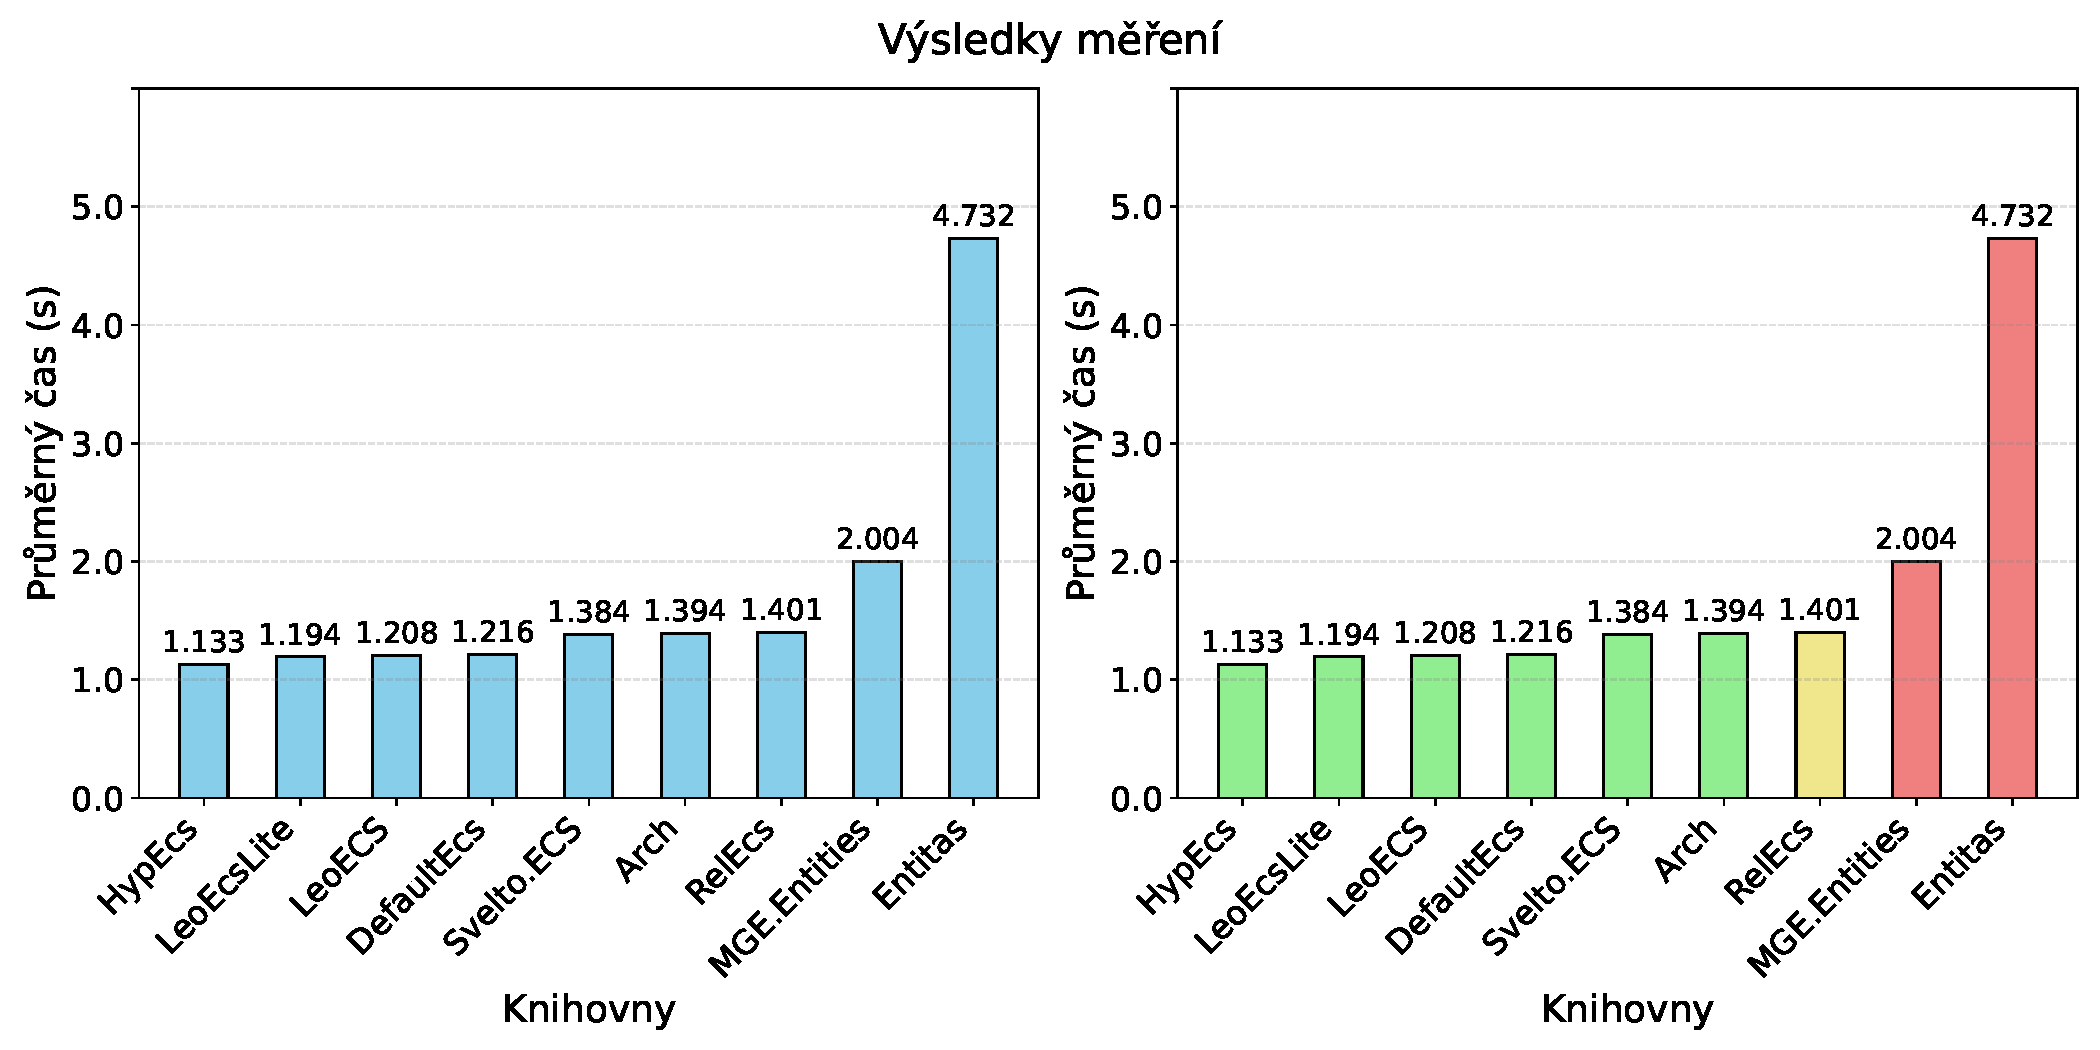
\includegraphics[width=1.0\linewidth]{plots/benchmark_results.pdf}
    \caption{Grafy vyobrazující výsledky měření zachycené v tabulce~\ref{tab:benchmark-results}. Pravý graf je obarven podle kategorií ze sekce~\ref{hypothesis}.}
    \label{fig:benchmark-results}
\end{figure}

V sekci~\ref{hypothesis} jsme si stanovili hypotézu, podle které mají nejlépe vyjít knihovny, které využívají \textit{archtype} (viz zelená barva). Nejhůře mají vyjít knihovny, které vyžadují aby komponenty byli třídy (viz červená barva). Mezi nimi se umístí knihovny, které kombinují obě vlastnosti (viz žlutá barva). Při nahlédnutí do tabulky~\ref{tab:benchmark-results} nebo grafu z obrázku~\ref{fig:benchmark-results} je lehké pozorovat, že tomu tak opravdu je. Ovšem je nutné podotknout, že knihovny \textit{Arch} a \textit{RelEcs} mají velmi podobný výsledek a pokud nahlédneme na chybu z tabulky~\ref{tab:benchmark-results} tak je možné pozorovat, že časy jsou téměř identické. Vyplyva z toho to, že požadavek na to, aby jednotlivé komponenty byli struktury, nemusí nutně vést k velkému výkonnostnímu zlepšení.

Zajímavou knihovnou je knihovna \textit{Svelto.ECS}, která vyžaduje aby bylo během kompilace známo z kterých komponent se jednotlivé entity budou skládat. Je lehké pozorovat že tato omezení nevedli k většímu výkonnostnímu zlepšení.

ECS knihovna \textit{Entitas} je na platformě GitHub~\cite{GitHub} nejpopulárnější (má nejvíce hvězdiček) ECS knihovnou pro C\#. I přesto, že v našem měření vyšla nejhůře její výkon je pořád dost dobrý. K její popularitě také přispívá větší podpora pro herní engine \textit{Unity}~\cite{Unity}.